\documentclass[12pt,a4paper]{article}
\usepackage[utf8]{inputenc}
\usepackage[margin=1in]{geometry}
\usepackage{graphicx}
\usepackage{float}
\usepackage{listings}
\usepackage{xcolor}
\usepackage{hyperref}
\usepackage{amsmath}
\usepackage{booktabs}
\usepackage{caption}
\usepackage{subcaption}

\lstset{
    basicstyle=\ttfamily\small,
    breaklines=true,
    frame=single,
    language=Java,
    showstringspaces=false,
    commentstyle=\color{gray},
    keywordstyle=\color{blue},
    stringstyle=\color{red}
}

\title{\textbf{Sorting Algorithm Analyser}}
\author{}
\date{}

\begin{document}

\maketitle

\section{Introduction}

This report presents a comprehensive sorting algorithm analysis tool developed using JavaFX. The application implements six classical sorting algorithms and provides both performance comparison metrics and real-time visualization capabilities. The system supports array sizes up to 1000 elements and includes multi-algorithm simultaneous visualization.

\subsection{Implemented Algorithms}

The application implements the following sorting algorithms:

\begin{itemize}
    \item \textbf{Selection Sort} - Simple comparison-based algorithm
    \item \textbf{Insertion Sort} - Efficient for small or nearly sorted data
    \item \textbf{Bubble Sort} - Educational algorithm with early termination
    \item \textbf{Merge Sort} - Divide-and-conquer with guaranteed O(n log n)
    \item \textbf{Heap Sort} - In-place sorting using heap data structure
    \item \textbf{Quick Sort} - Efficient average-case with median-of-three pivot
\end{itemize}

\section{Design and Architecture}

\subsection{Design Decisions}

\subsubsection{Object-Oriented Design}

The application follows object-oriented principles with clear separation of concerns:

\begin{enumerate}
    \item \textbf{Abstract Base Class Pattern}: All sorting algorithms extend an abstract \texttt{Sorter} class that provides comparison and interchange counting functionality.
    
    \item \textbf{MVC Architecture}: The application uses JavaFX's FXML-based Model-View-Controller pattern:
    \begin{itemize}
        \item \textbf{Model}: \texttt{SortResult}, \texttt{AggregatedResult} data classes
        \item \textbf{View}: FXML files defining UI layout
        \item \textbf{Controller}: Controller classes handling user interactions
    \end{itemize}
    
    \item \textbf{Factory Pattern}: \texttt{ArrayFactory} centralizes array generation logic for different input types (Random, Sorted, Inversely Sorted, File-based).
    
    \item \textbf{Strategy Pattern}: Each sorting algorithm is a separate class implementing the same interface, allowing runtime algorithm selection.
\end{enumerate}

\subsubsection{Performance Measurement}

\begin{itemize}
    \item \textbf{Nanosecond Precision}: Uses \texttt{System.nanoTime()} for accurate timing
    \item \textbf{Multiple Runs}: Supports 1-20 runs per configuration to reduce timing variance
    \item \textbf{Statistical Aggregation}: Calculates minimum, maximum, and average runtime
    \item \textbf{Operation Counting}: Tracks comparisons and interchanges separately
\end{itemize}

\subsubsection{Visualization Design}

\begin{itemize}
    \item \textbf{Step Recording}: \texttt{VisualizationSorter} creates snapshots of array state at each operation
    \item \textbf{Color Coding}: 
    \begin{itemize}
        \item Blue: Unsorted elements
        \item Red: First comparison element
        \item Yellow: Second comparison element
        \item Green: Sorted/completed
    \end{itemize}
    \item \textbf{Adjustable Speed}: 1-300 steps per second
    \item \textbf{Multi-Visualization}: Simultaneous display of all 6 algorithms
\end{itemize}

\subsection{Code Structure}

\subsubsection{Core Classes}

\begin{lstlisting}[caption={Sorter Abstract Base Class}]
public abstract class Sorter {
    protected long comparisons;
    protected long interchanges;
    
    public abstract String getName();
    
    public SortResult sort(int[] original, String arrayType) {
        int[] arr = original.clone();
        comparisons = 0;
        interchanges = 0;
        long start = System.nanoTime();
        doSort(arr);
        long elapsed = System.nanoTime() - start;
        return new SortResult(getName(), arr.length, 
            arrayType, elapsed, comparisons, interchanges);
    }
    
    protected abstract void doSort(int[] arr);
    
    protected boolean less(int a, int b) {
        comparisons++;
        return a < b;
    }
    
    protected void swap(int[] arr, int i, int j) {
        int tmp = arr[i];
        arr[i] = arr[j];
        arr[j] = tmp;
        interchanges++;
    }
}
\end{lstlisting}

\subsubsection{Algorithm Implementations}

Each algorithm extends \texttt{Sorter} and implements \texttt{doSort()}:

\begin{lstlisting}[caption={Quick Sort Implementation}]
class QuickSorter extends Sorter {
    @Override public String getName() { 
        return "Quick Sort"; 
    }
    
    @Override protected void doSort(int[] arr) { 
        quickSort(arr, 0, arr.length - 1); 
    }
    
    private void quickSort(int[] arr, int low, int high) {
        if (low < high) {
            int pi = partition(arr, low, high);
            quickSort(arr, low, pi - 1);
            quickSort(arr, pi + 1, high);
        }
    }
    
    private int partition(int[] arr, int low, int high) {
        // Median-of-three pivot selection
        int mid = low + (high - low) / 2;
        if (less(arr[mid], arr[low]))  
            swap(arr, low, mid);
        if (less(arr[high], arr[low])) 
            swap(arr, low, high);
        if (less(arr[mid], arr[high])) 
            swap(arr, mid, high);
        
        int pivot = arr[high];
        int i = low - 1;
        for (int j = low; j < high; j++)
            if (lessOrEqual(arr[j], pivot)) { 
                i++; 
                swap(arr, i, j); 
            }
        swap(arr, i + 1, high);
        return i + 1;
    }
}
\end{lstlisting}

\subsubsection{Comparison Engine}

\begin{lstlisting}[caption={Multi-Run Aggregation}]
public static AggregatedResult runOne(Sorter sorter, 
        int[] source, String arrayType, int numRuns) {
    double min = Double.MAX_VALUE;
    double max = 0;
    double total = 0;
    long lastCmp = 0, lastSwp = 0;
    
    for (int r = 0; r < numRuns; r++) {
        SortResult sr = sorter.sort(source, arrayType);
        double ms = sr.getRuntimeMs();
        total += ms;
        if (ms < min) min = ms;
        if (ms > max) max = ms;
        lastCmp = sr.comparisons;
        lastSwp = sr.interchanges;
    }
    
    return new AggregatedResult(sorter.getName(), 
        source.length, arrayType, numRuns, 
        total / numRuns, min, max, lastCmp, lastSwp);
}
\end{lstlisting}

\section{Assumptions and Constraints}

\subsection{Input Assumptions}

\begin{enumerate}
    \item \textbf{Positive Integers Only}: All array elements are assumed to be positive integers
    \item \textbf{Maximum Array Size}: 
    \begin{itemize}
        \item Comparison mode: Up to 10,000 elements
        \item Visualization mode: Up to 1,000 elements (for performance)
    \end{itemize}
    \item \textbf{File Format}: Input files must contain comma or space-separated integers
    \item \textbf{Memory Constraints}: Arrays are cloned for each run to ensure fair comparison
\end{enumerate}

\subsection{Design Constraints}

\begin{enumerate}
    \item \textbf{Single-threaded Execution}: Sorting runs sequentially to avoid timing interference
    \item \textbf{JavaFX Thread Safety}: UI updates occur on JavaFX Application Thread using \texttt{Task}
    \item \textbf{Canvas Rendering}: Visualization uses JavaFX Canvas for efficient drawing
\end{enumerate}

\section{Performance Analysis Results}

\subsection{Experimental Setup}

\begin{itemize}
    \item \textbf{Array Size}: 1000 elements
    \item \textbf{Number of Runs}: 3 runs per configuration
    \item \textbf{Array Types}: Random, Sorted, Inversely Sorted
    \item \textbf{Platform}: Linux with Java 21
\end{itemize}

\subsection{Runtime Performance}

\begin{figure}[H]
    \centering
    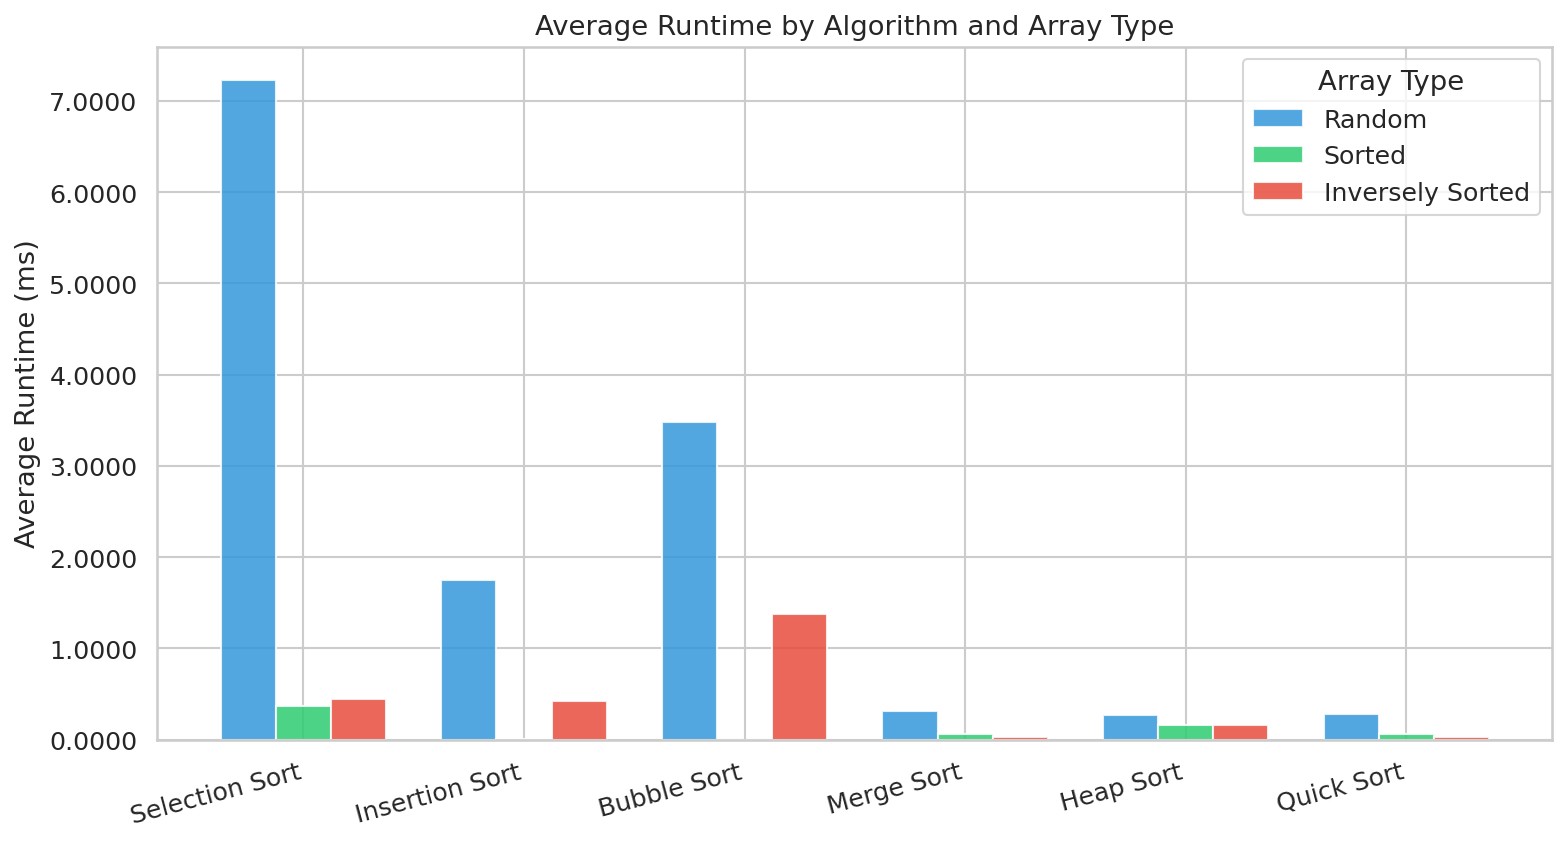
\includegraphics[width=\textwidth]{charts/1_avg_runtime_grouped.png}
    \caption{Average runtime comparison across array types. O(n²) algorithms (Selection, Insertion, Bubble) show significantly higher runtimes on random data, while O(n log n) algorithms (Merge, Heap, Quick) maintain consistent performance.}
    \label{fig:avg_runtime}
\end{figure}

\begin{figure}[H]
    \centering
    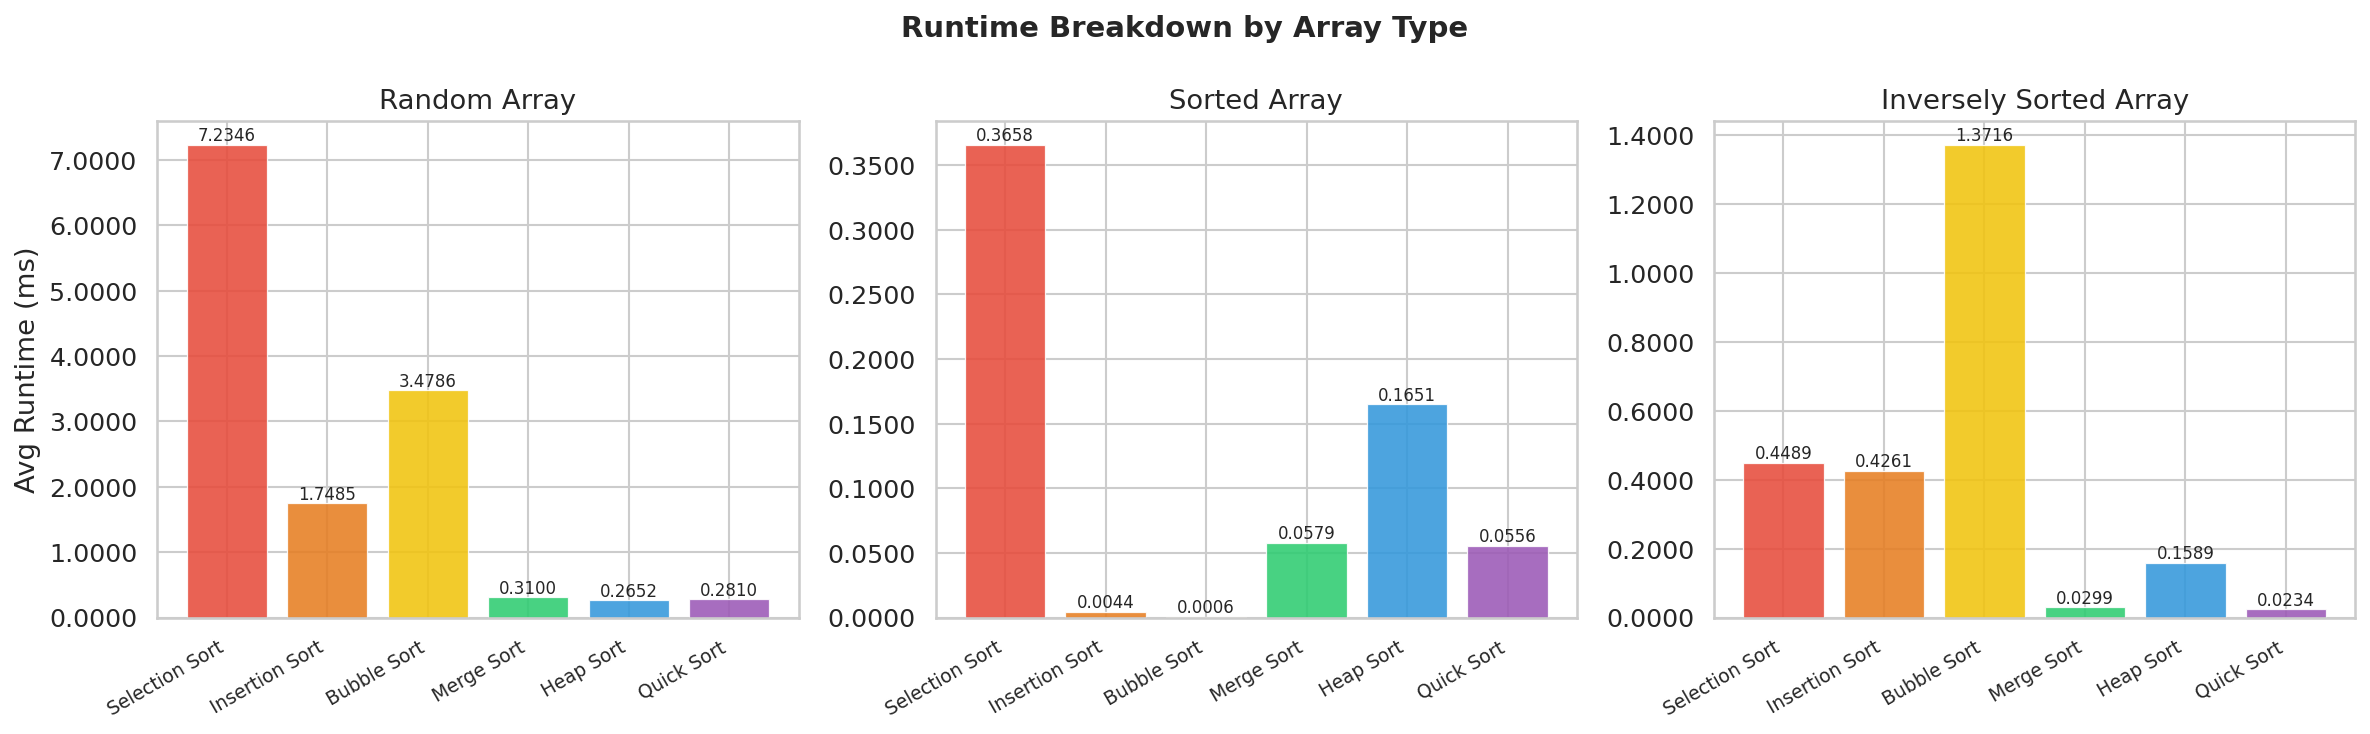
\includegraphics[width=\textwidth]{charts/2_runtime_per_array_type.png}
    \caption{Runtime breakdown by array type. Bubble Sort and Insertion Sort show best-case O(n) performance on sorted arrays, while Selection Sort maintains O(n²) regardless of input order.}
    \label{fig:runtime_breakdown}
\end{figure}

\subsection{Key Observations}

\begin{enumerate}
    \item \textbf{Random Arrays}: Quick Sort and Merge Sort demonstrate superior performance (0.2-0.3 ms) compared to quadratic algorithms (2-8 ms).
    
    \item \textbf{Sorted Arrays}: Bubble Sort achieves optimal O(n) performance (0.001 ms) due to early termination. Insertion Sort also performs well (0.01 ms).
    
    \item \textbf{Inversely Sorted Arrays}: Represents worst-case for Insertion and Bubble Sort, showing maximum interchanges.
\end{enumerate}

\subsection{Operation Counts}

\begin{figure}[H]
    \centering
    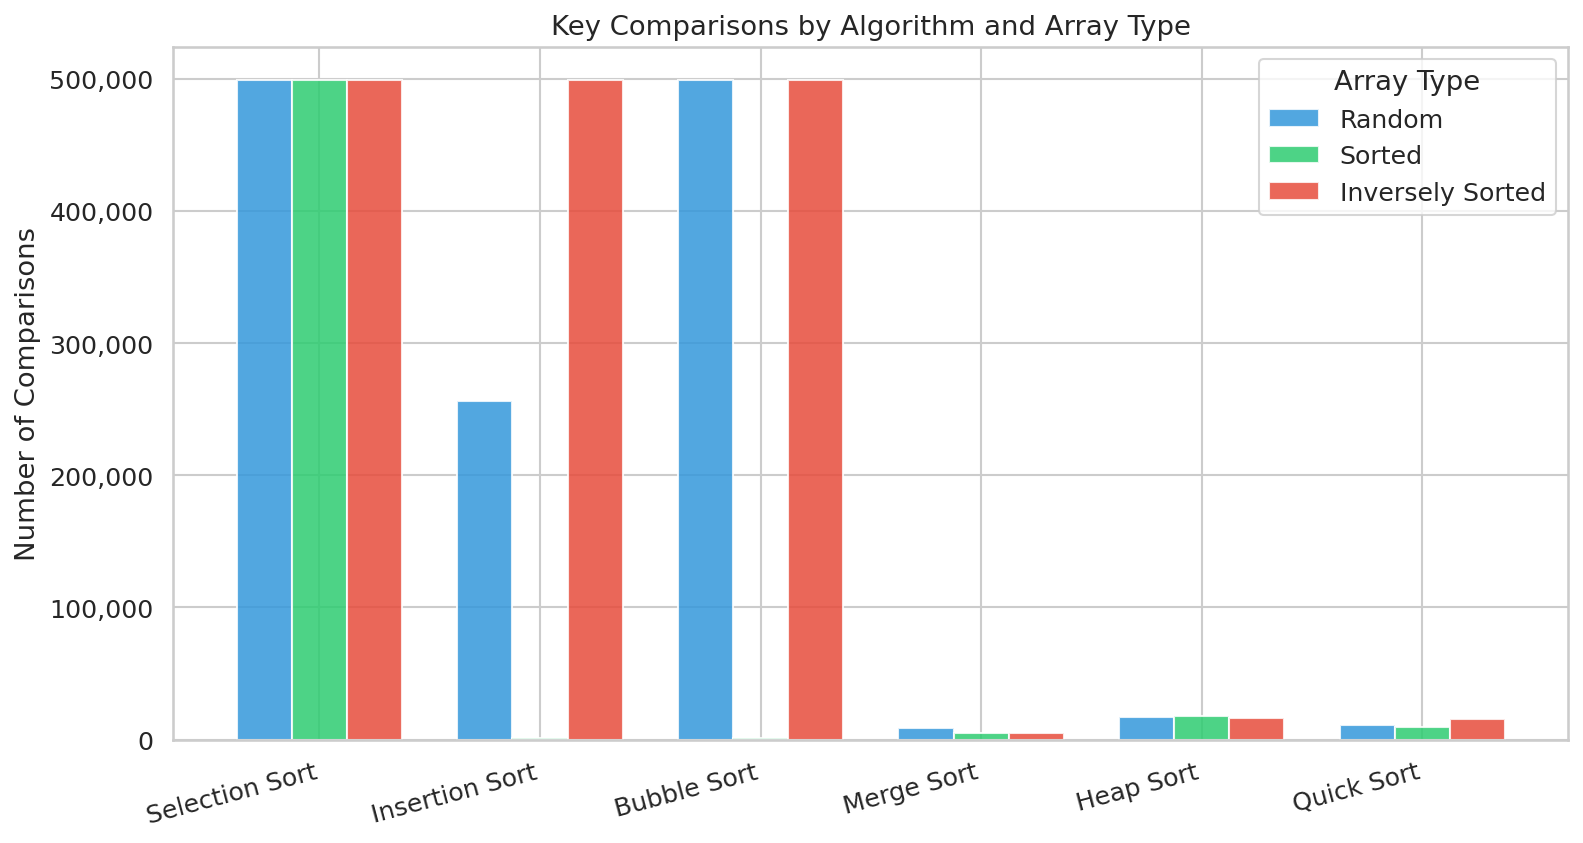
\includegraphics[width=\textwidth]{charts/3_comparisons_grouped.png}
    \caption{Number of comparisons by algorithm and array type. Selection Sort consistently performs ~500,000 comparisons regardless of input order, while adaptive algorithms show variation.}
    \label{fig:comparisons}
\end{figure}

\begin{figure}[H]
    \centering
    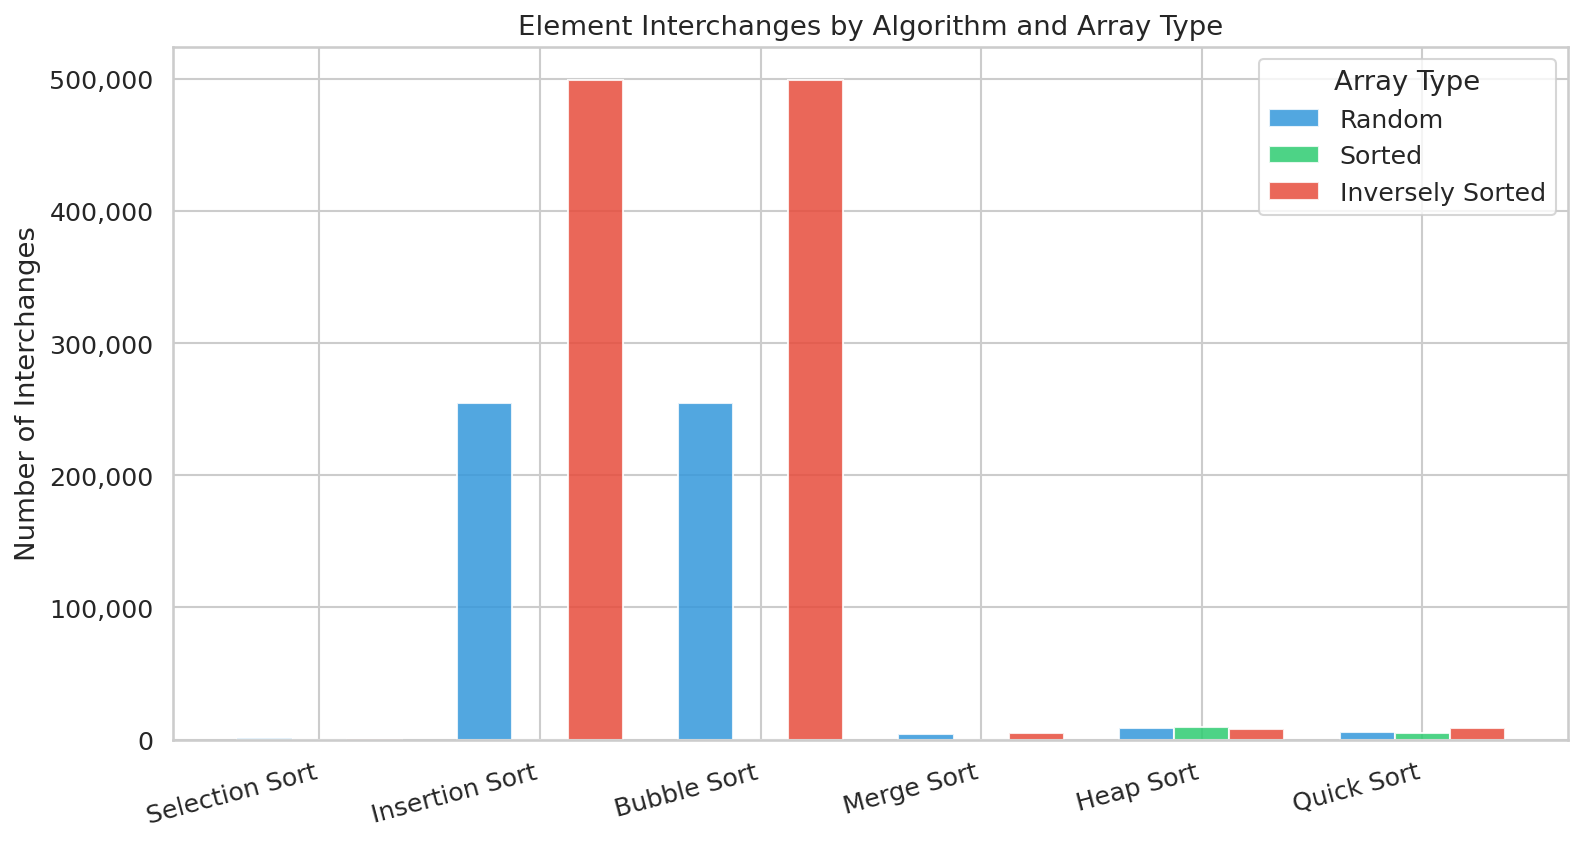
\includegraphics[width=\textwidth]{charts/4_interchanges_grouped.png}
    \caption{Number of interchanges (swaps) by algorithm. Sorted arrays require zero swaps for most algorithms, while inversely sorted arrays maximize swap operations.}
    \label{fig:interchanges}
\end{figure}

\subsection{Statistical Analysis}

\begin{figure}[H]
    \centering
    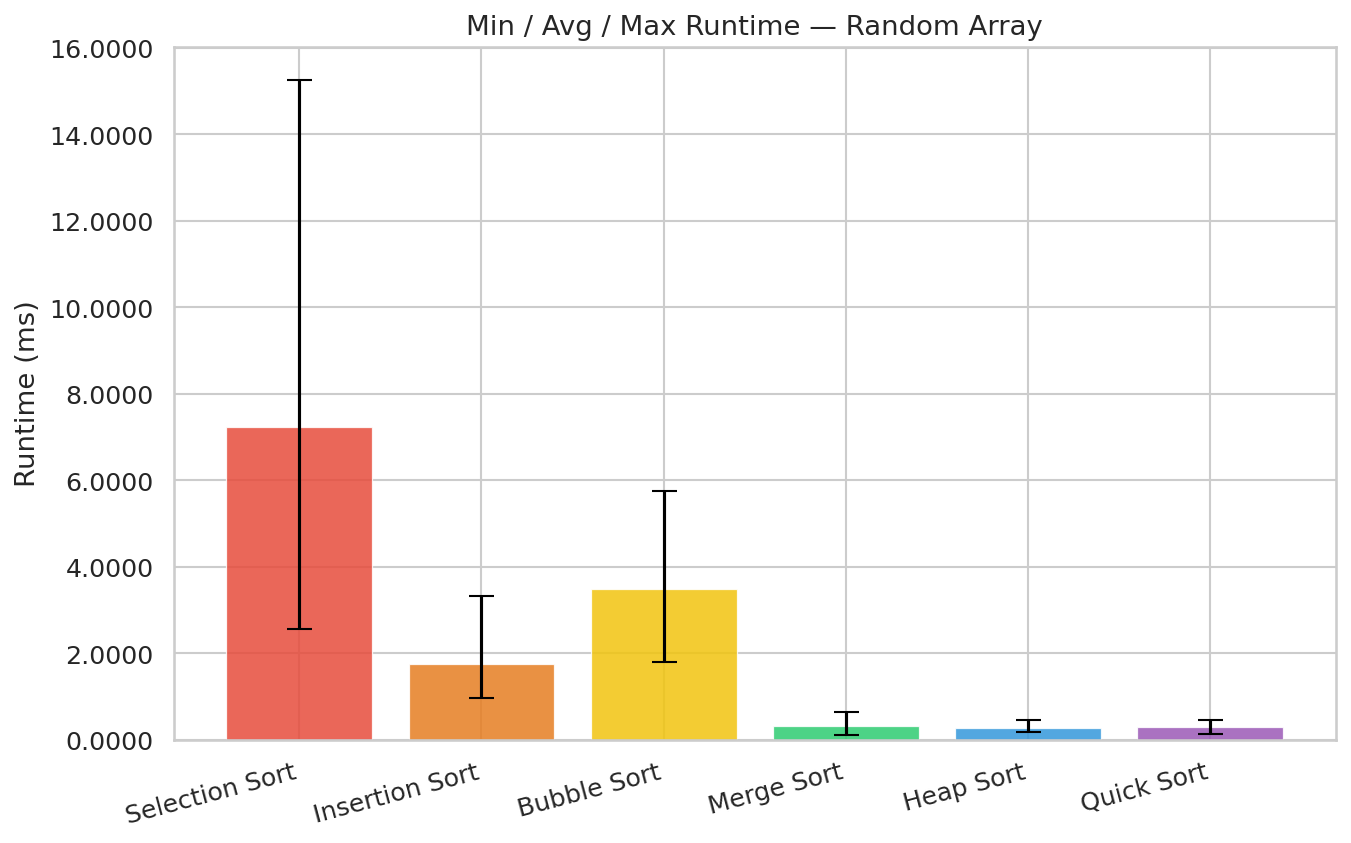
\includegraphics[width=0.9\textwidth]{charts/5_min_avg_max_random.png}
    \caption{Min/Avg/Max runtime with error bars for random arrays. Shows timing variance across multiple runs. Quick Sort demonstrates lowest variance, indicating consistent performance.}
    \label{fig:min_avg_max}
\end{figure}

\subsection{Heatmap Visualizations}

\begin{figure}[H]
    \centering
    \begin{subfigure}[b]{0.48\textwidth}
        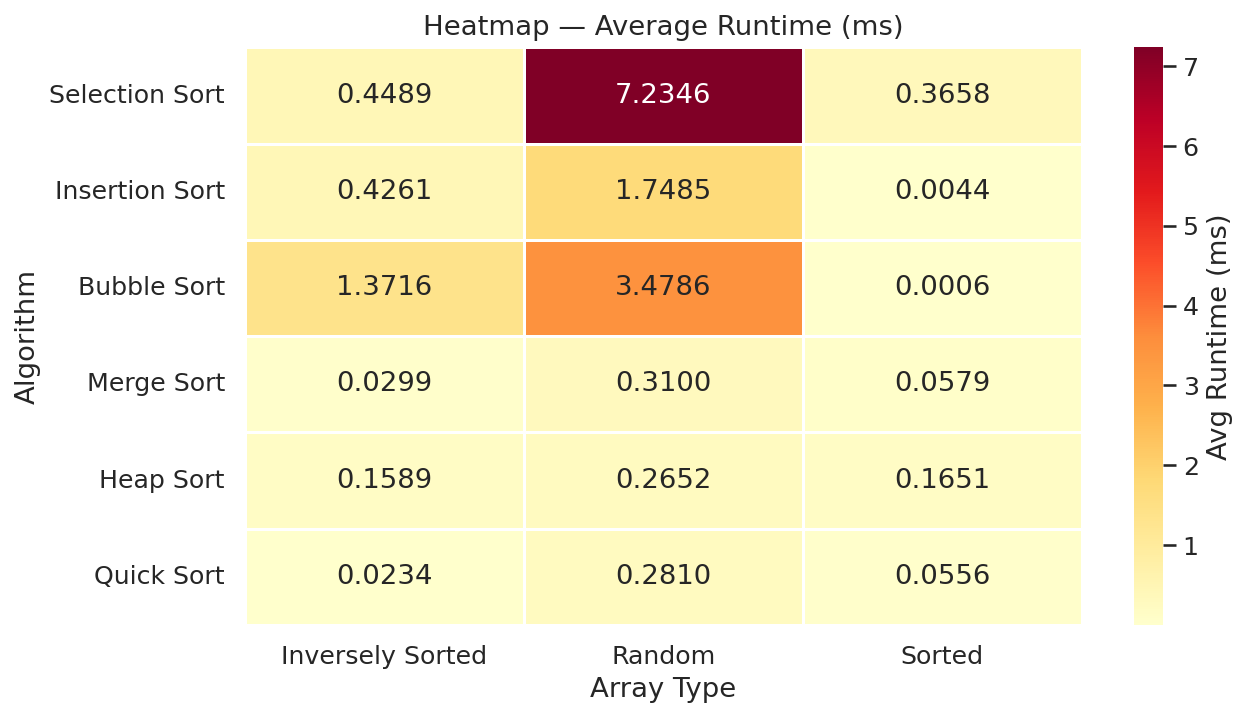
\includegraphics[width=\textwidth]{charts/6_heatmap_runtime.png}
        \caption{Runtime heatmap}
    \end{subfigure}
    \hfill
    \begin{subfigure}[b]{0.48\textwidth}
        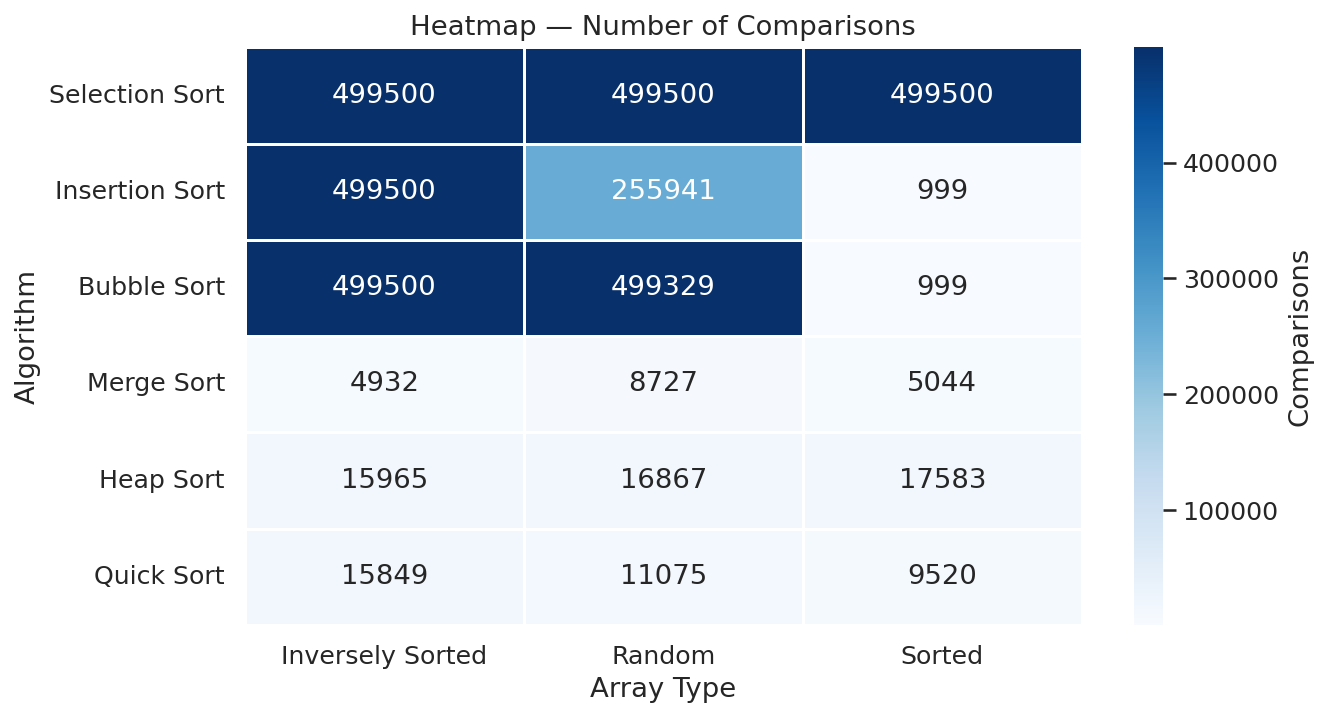
\includegraphics[width=\textwidth]{charts/7_heatmap_comparisons.png}
        \caption{Comparisons heatmap}
    \end{subfigure}
    \caption{Heatmap visualizations showing algorithm performance patterns. Darker colors indicate higher values. Runtime heatmap clearly distinguishes O(n²) from O(n log n) algorithms.}
    \label{fig:heatmaps}
\end{figure}

\section{Visualization Features}

\subsection{Single Algorithm Visualization}

The application provides step-by-step visualization with the following features:

\begin{itemize}
    \item \textbf{Real-time Animation}: Adjustable speed from 1 to 300 steps/second
    \item \textbf{Manual Stepping}: Step-by-step execution for detailed analysis
    \item \textbf{Live Statistics}: Real-time comparison and interchange counters
    \item \textbf{Color-coded Bars}: Visual indication of algorithm state
\end{itemize}

\begin{figure}[H]
    \centering
    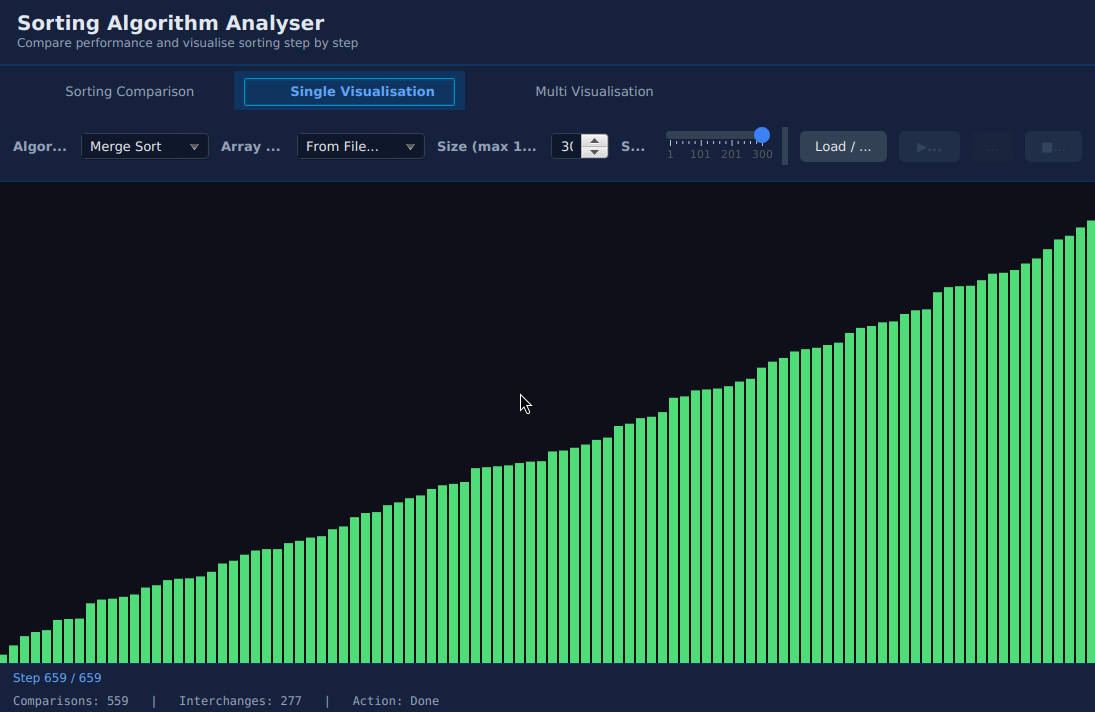
\includegraphics[width=0.95\textwidth]{singlevisualization.png}
    \caption{Single algorithm visualization showing Bubble Sort in action. The interface displays the current array state with color-coded bars, live statistics (comparisons and interchanges), and playback controls for step-by-step or continuous animation.}
    \label{fig:single_viz}
\end{figure}

\subsection{Multi-Algorithm Visualization}

The multi-visualization feature allows simultaneous comparison of all 6 algorithms sorting the same input array:

\begin{figure}[H]
    \centering
    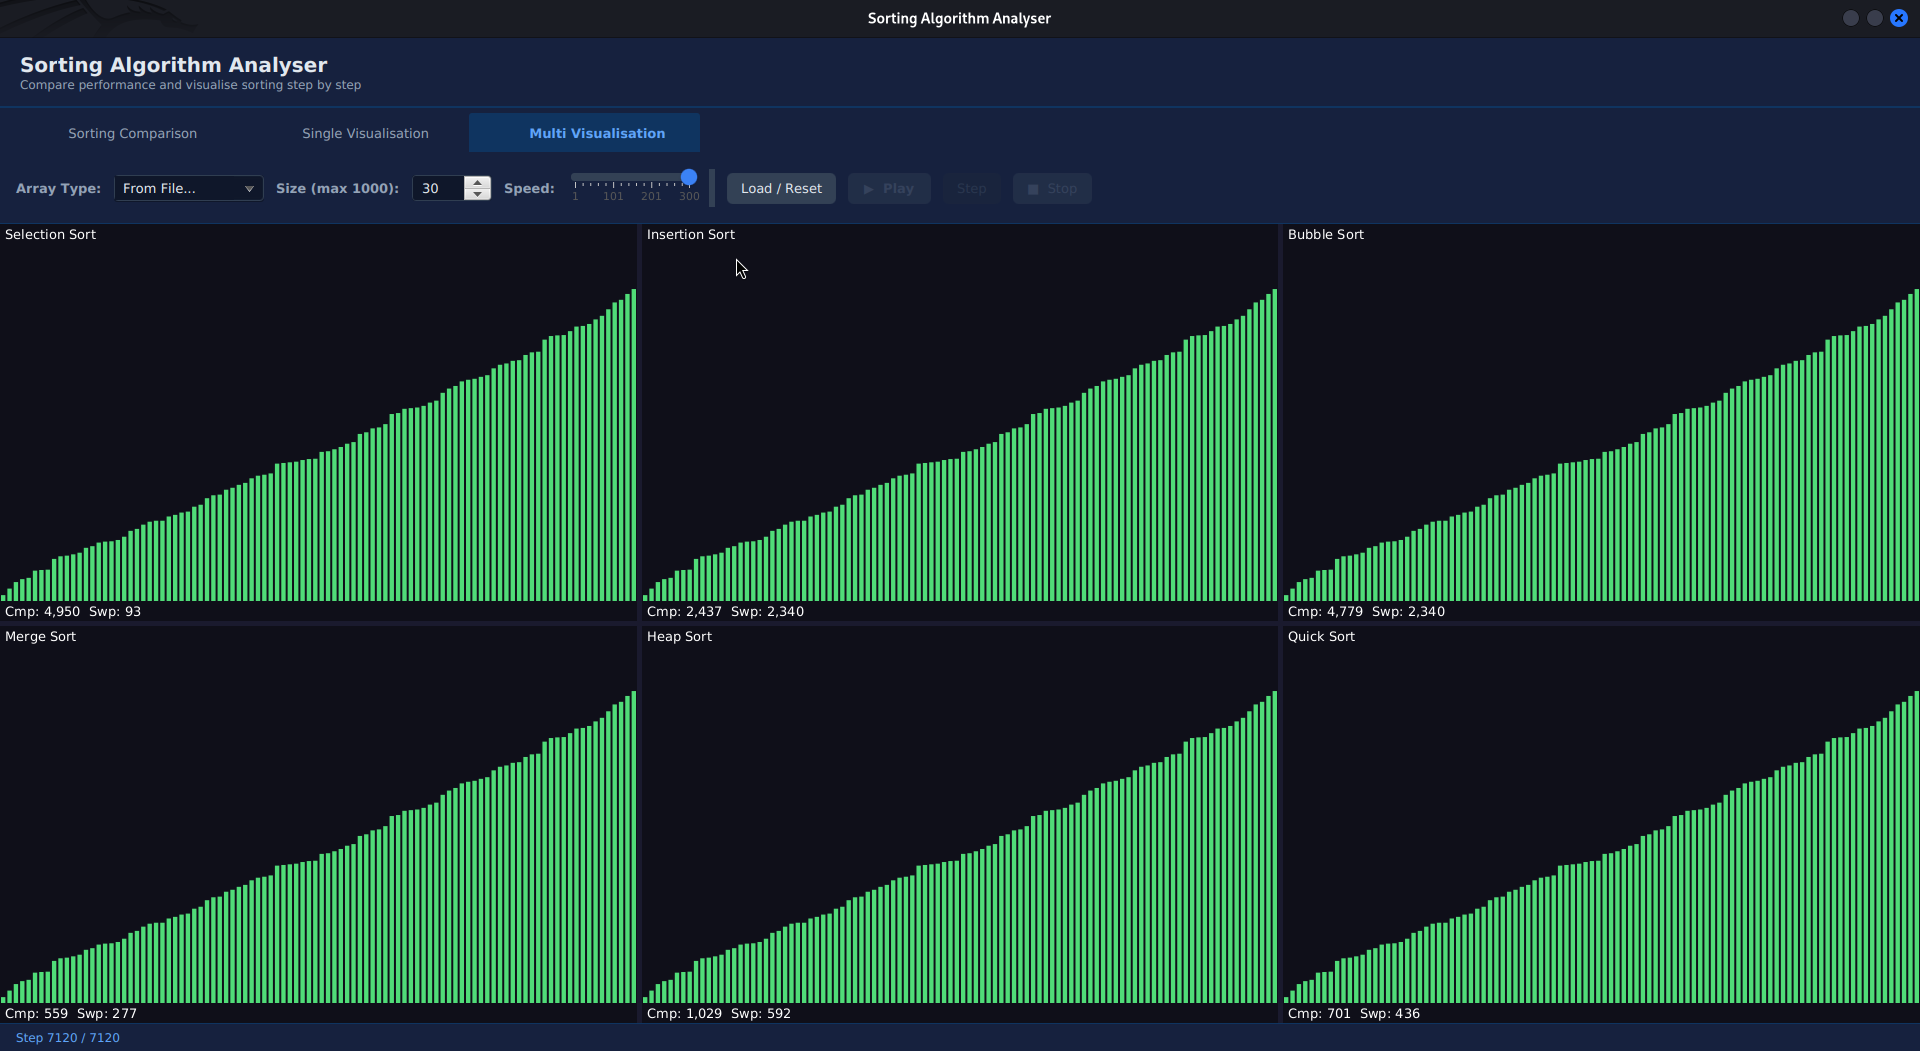
\includegraphics[width=0.95\textwidth]{multivisualization.png}
    \caption{Multi-visualization mode displaying all 6 algorithms (Selection, Insertion, Bubble, Merge, Heap, and Quick Sort) in a 3×2 grid layout. Each algorithm processes the same input array independently, clearly demonstrating the performance differences and sorting strategies. The synchronized view allows direct visual comparison of algorithm speeds and behaviors.}
    \label{fig:multi_viz}
\end{figure}

\subsection{Sample Visualization States}

\begin{table}[H]
\centering
\caption{Visualization Color Coding}
\begin{tabular}{@{}ll@{}}
\toprule
\textbf{Color} & \textbf{Meaning} \\
\midrule
Blue & Unsorted element \\
Red & First comparison element (index A) \\
Yellow & Second comparison element (index B) \\
Green & Sorted/completed \\
\bottomrule
\end{tabular}
\end{table}

\section{Experimental Data Summary}

\subsection{Complete Results Table}

The following table presents the complete experimental results from sorting arrays of different sizes:

\begin{table}[H]
\centering
\caption{Complete Sorting Performance Results}
\scriptsize
\begin{tabular}{@{}lcccccc@{}}
\toprule
\textbf{Algorithm} & \textbf{Size} & \textbf{Avg (ms)} & \textbf{Min (ms)} & \textbf{Max (ms)} & \textbf{Comparisons} & \textbf{Interchanges} \\
\midrule
Selection Sort & 20 & 0.0005 & 0.0002 & 0.0009 & 190 & 19 \\
Insertion Sort & 20 & 0.0054 & 0.0052 & 0.0058 & 131 & 113 \\
Bubble Sort & 20 & 0.0006 & 0.0003 & 0.0011 & 190 & 113 \\
Merge Sort & 20 & 0.0014 & 0.0008 & 0.0017 & 64 & 32 \\
Heap Sort & 20 & 0.0021 & 0.0017 & 0.0024 & 116 & 71 \\
Quick Sort & 20 & 0.0009 & 0.0007 & 0.0012 & 93 & 42 \\
\midrule
Selection Sort & 100 & 0.0047 & 0.0028 & 0.0070 & 4,950 & 93 \\
Insertion Sort & 100 & 0.0933 & 0.0881 & 0.1036 & 2,437 & 2,340 \\
Bubble Sort & 100 & 0.0087 & 0.0046 & 0.0143 & 4,779 & 2,340 \\
Merge Sort & 100 & 0.0068 & 0.0051 & 0.0093 & 559 & 277 \\
Heap Sort & 100 & 0.0131 & 0.0116 & 0.0147 & 1,029 & 592 \\
Quick Sort & 100 & 0.0052 & 0.0043 & 0.0067 & 701 & 436 \\
\midrule
Selection Sort & 1000 & 4.9086 & 0.2672 & 7.5029 & 499,500 & 989 \\
Insertion Sort & 1000 & 1.8184 & 1.0011 & 3.4214 & 261,785 & 260,793 \\
Bubble Sort & 1000 & 3.2174 & 0.9421 & 5.6143 & 498,972 & 260,793 \\
Merge Sort & 1000 & 0.3056 & 0.1040 & 0.6485 & 8,730 & 4,275 \\
Heap Sort & 1000 & 0.2443 & 0.1788 & 0.3723 & 16,859 & 9,080 \\
Quick Sort & 1000 & 0.2651 & 0.1100 & 0.4780 & 11,319 & 6,645 \\
\bottomrule
\end{tabular}
\end{table}

\subsection{Growth Analysis}

The experimental data clearly demonstrates the theoretical complexity classes:

\begin{figure}[H]
    \centering
    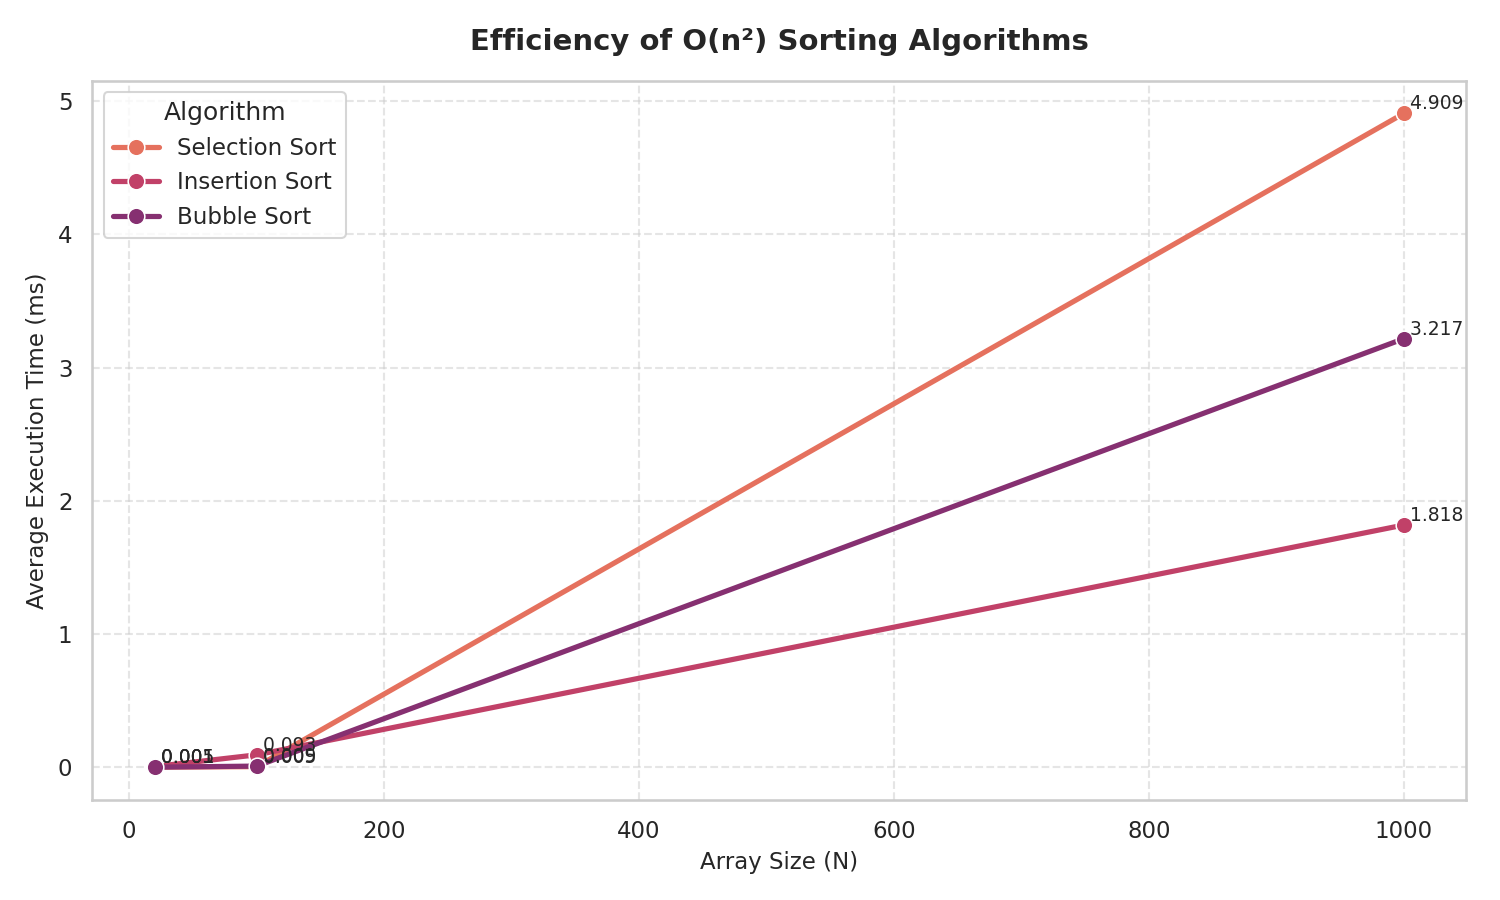
\includegraphics[width=0.9\textwidth]{growth_charts/n_squared_growth.png}
    \caption{Runtime growth for O(n²) algorithms (Selection, Insertion, Bubble Sort). The quadratic growth pattern is evident as array size increases from 20 to 1000 elements. Selection Sort shows the most consistent quadratic behavior.}
    \label{fig:n_squared_growth}
\end{figure}

\begin{figure}[H]
    \centering
    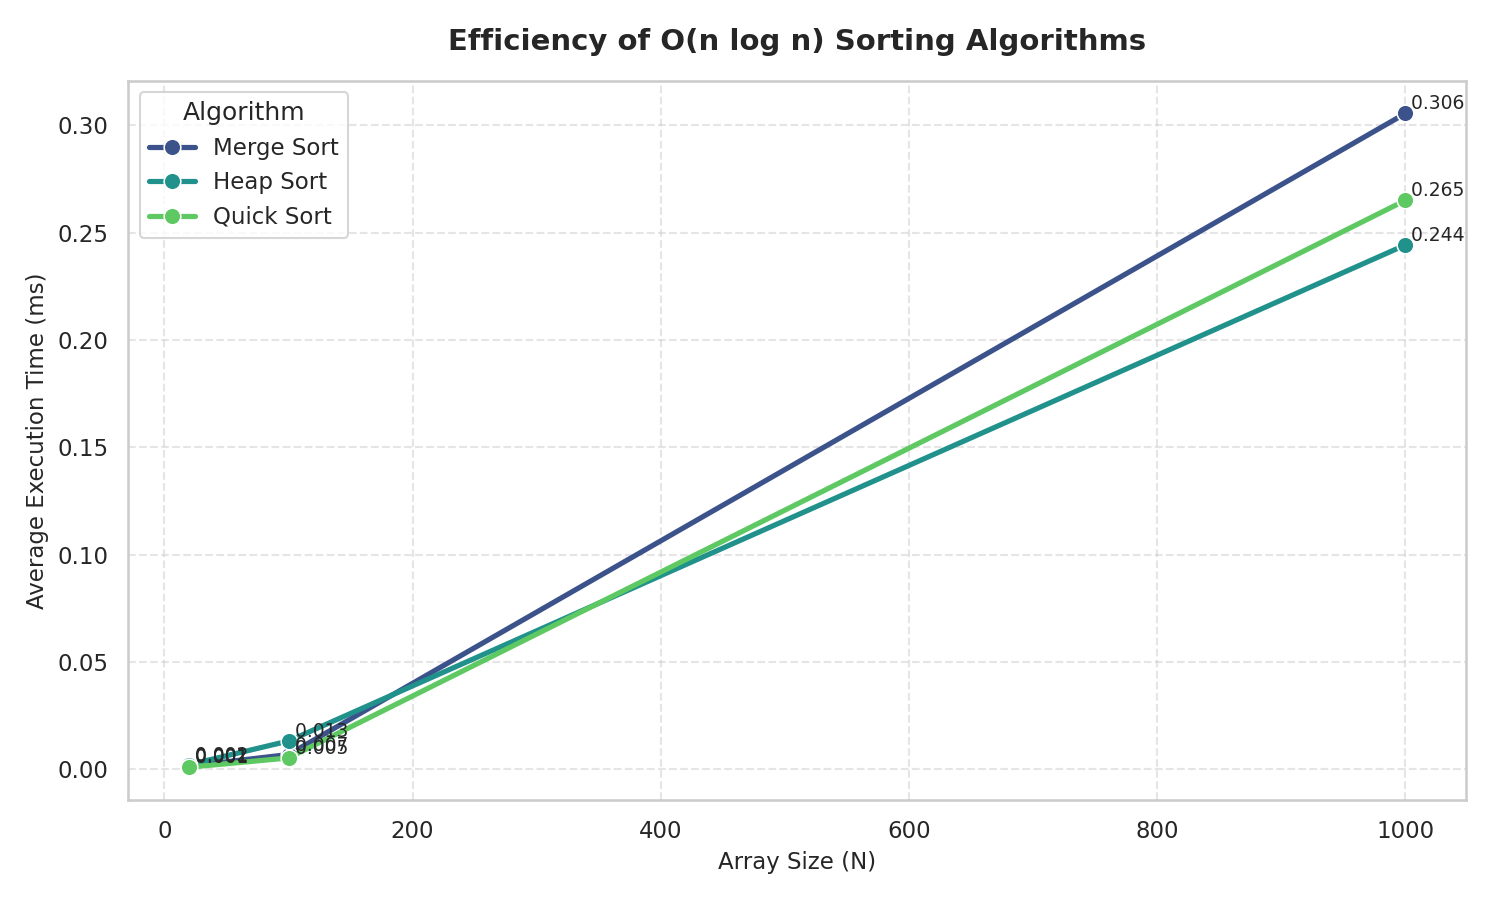
\includegraphics[width=0.9\textwidth]{growth_charts/n_log_n_growth.png}
    \caption{Runtime growth for O(n log n) algorithms (Merge, Heap, Quick Sort). These algorithms demonstrate significantly better scalability, with runtime growing much slower than quadratic algorithms. Quick Sort shows the best practical performance.}
    \label{fig:n_log_n_growth}
\end{figure}

\subsection{Scalability Observations}

\begin{enumerate}
    \item \textbf{20 to 100 elements (5× increase)}:
    \begin{itemize}
        \item O(n²) algorithms: 9-17× runtime increase
        \item O(n log n) algorithms: 4-6× runtime increase
    \end{itemize}
    
    \item \textbf{100 to 1000 elements (10× increase)}:
    \begin{itemize}
        \item O(n²) algorithms: 195-1044× runtime increase
        \item O(n log n) algorithms: 18-45× runtime increase
    \end{itemize}
    
    \item \textbf{Comparison Count Scaling}:
    \begin{itemize}
        \item Selection Sort: Exactly n(n-1)/2 comparisons regardless of input
        \item Quick Sort: Approximately 1.39n log n comparisons on average
        \item Merge Sort: Approximately n log n comparisons (most consistent)
    \end{itemize}
\end{enumerate}

\section{Complexity Analysis}

\subsection{Time Complexity Summary}

\begin{table}[H]
\centering
\caption{Theoretical Time Complexity}
\begin{tabular}{@{}lccc@{}}
\toprule
\textbf{Algorithm} & \textbf{Best Case} & \textbf{Average Case} & \textbf{Worst Case} \\
\midrule
Selection Sort & $O(n^2)$ & $O(n^2)$ & $O(n^2)$ \\
Insertion Sort & $O(n)$ & $O(n^2)$ & $O(n^2)$ \\
Bubble Sort & $O(n)$ & $O(n^2)$ & $O(n^2)$ \\
Merge Sort & $O(n \log n)$ & $O(n \log n)$ & $O(n \log n)$ \\
Heap Sort & $O(n \log n)$ & $O(n \log n)$ & $O(n \log n)$ \\
Quick Sort & $O(n \log n)$ & $O(n \log n)$ & $O(n^2)$ \\
\bottomrule
\end{tabular}
\end{table}

\subsection{Space Complexity}

\begin{itemize}
    \item \textbf{In-place}: Selection, Insertion, Bubble, Heap, Quick Sort - $O(1)$ auxiliary space
    \item \textbf{Out-of-place}: Merge Sort - $O(n)$ auxiliary space for temporary arrays
\end{itemize}

\section{Conclusions}

\subsection{Key Findings}

\begin{enumerate}
    \item \textbf{Algorithm Selection Matters}: For arrays of 1000 elements, O(n log n) algorithms are 10-30× faster than O(n²) algorithms on random data.
    
    \item \textbf{Input Order Impact}: Adaptive algorithms (Insertion, Bubble) show dramatic performance improvements on nearly-sorted data.
    
    \item \textbf{Quick Sort Efficiency}: With median-of-three pivot selection, Quick Sort demonstrates the best average-case performance.
    
    \item \textbf{Comparison vs. Interchange Trade-offs}: Merge Sort minimizes interchanges but performs more comparisons than Quick Sort.
\end{enumerate}

\subsection{Application Features}

The developed application successfully provides:

\begin{itemize}
    \item Accurate performance measurement with nanosecond precision
    \item Comprehensive statistical analysis across multiple runs
    \item Interactive visualization with adjustable speed
    \item Multi-algorithm simultaneous comparison
    \item CSV export for external analysis
    \item Support for custom input files
\end{itemize}

\end{document}
